\chapter{Literature Review}

\section{The need for performing brake tests}
The brake system is a critical part of an automobile, thanks to this system it is possible to use the latter under safe conditions both in urban and rural areas. There are some ideal requirements that a brake system should be able to attend \cite{kawaguchi} :

\begin{itemize}
	\item Reduce the speed of a moving vehicle, increasing the deceleration of the same.
	\item Stop the vehicle completely.
	\item Maintain the vehicle speed, preventing unwanted acceleration in downhill paths.
	\item Keep the vehicle motionless while it is parked.
\end{itemize}

It is important to emphasize that this conditions are ideal, considering that in extremely hazardous or stressful situations the system might not operate properly and will not attend thoose previous requirementes. Considering the importance of brake system the same need to have minimal breaking capacity so vehicles can be decelerated with greater efficience. 
\par
In contrast, more effective brake systems means more cost to manufactures and consenquently to customers. Theoretically this would meant that manufactures need to choose a trade-off between quality and cost. However, the point in which this trade-off is setted is determined by governament regulations. Moreover if there was no general regulations each car manufecturer would have a standard that they judge is sufficient. In Brazil the governament partitions that define this regulations are the \textit{National Traffic Council} and the \textit{National Institute of Meteorology, Quality and Technology}, most of those regulations are based in the european regulation ECE-13/05 \cite{inmetro2013} .
\par
Considering the importance of regulatory standards, the need for brake tests becomes even more evident as it is mandatory to ensure that brake-systems will attend to regulations requirementes. Only with extensive testing it is possible to ensure that a particular system will attend to all standards regarding it's category of operation. 
\par
Making all theese considerations, a \textit{Break-System-Testbench} may be considered a useful device for the automotive industry. Considering that it would be able to simulate a close enough replica of real evironments and situations that a brake system is submitted, this testbench could allow car manufactures and break system parts manufactures to avoid expenses in tests as they would be able to test different parts of the system in a assisted and controlled evironment.


\section{Working principles of disk brake systems}

This section will give a short explanation of how disk breaks works as the vast majority of cars and motorcycles nowadays are equiped with this technology instead of the outdated drum scheme.
\par
In general terms we can make an analogy of how disk brake works with how bicycles brakes works. In a bicycle the brake calipers squeeze the wheels in order to promove deceleration to the wheel and reduce the bike speed. In disk breaks the calipers apply pressure to the rotor \textit{disk}, the rotor is directly connected to the wheel spinning at the same speed, this way the system decelerates the rotor and the wheel trying to reduce the vehicle speed. In car disk breaks there is a component called pad, as seen on Figure \ref{working-of-disk-breaks} pads are located between the calipers and the rotor. Pads have the functionality to reduce the wear generated by friction in the rotor. In normal conditions during proper maintenance calipers are hardly-ever replaced, pads are replaced every once in a while and disks are replaced also every once in a while but less frequently than pads.

\begin{figure}[htbp]
	\centering
		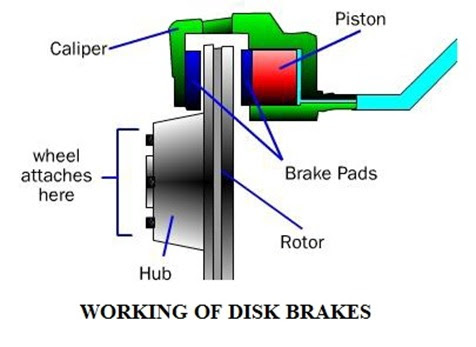
\includegraphics[scale=0.55]{figuras/disk_brake_working}
	\caption{Schematic for disk brake systems  \cite{working-of-disk-breaks} }
	\label{working-of-disk-breaks}
\end{figure}



\section{Monitored parameters}
As metioned before this paper will be based in the \textit{SAE J2522} regulations, this regulation says that to evaluate the efficiency of a brake system it is mandatory to monitor temperature on the brake pads, the pressure applied on the disk and the speed of the rotor throughout all the process. Monitoring the vibration is not mandatory but has some advantages.

\begin{itemize}
	\item\textit{Temperature of brake pads: } During all test it is mandatory to have full knowledge of the temperature of the break pads, firtly because of security reasons (there is upper limit for temperatura in any system) and also because of the wear of parts that is related to temperature.
	\item\textit{Pressure applied on the disks: } Knowing the magnitude of this force means being able to relate the pressure applied and the deceleration, knowing how the pressure applied increases the temperature of the pads and evaluate how this promotes wear of the parts.
	\item\textit{Rotation speed: } Without knowing how the speed of the rotor varies over time it would be impossible to determine the acceleration and deceleration rates among many other issues.
	\item\textit{Vibration: } As mentioned before this is not mandatory but rather interesting, measuring vibration makes it possible to determine how the extensive use can wear out the parts and reduce stiffness among other properties. Also it is natural that the system will vibrate during braking, minimal vibration or too much vibration can indicate a fault that on the future could damage the system.
\end{itemize}
